\documentclass{article}

% MATHS
\usepackage{amsmath}
\usepackage{gensymb}

\usepackage{mathtools}
\newcommand\coolover[2]{\mathrlap{\smash{\overbrace{\phantom{%
    \begin{matrix} #2 \end{matrix}}}^{\mbox{$#1$}}}}#2} 
\newcommand\coolunder[2]{\mathrlap{\smash{\underbrace{\phantom{%
    \begin{matrix} #2 \end{matrix}}}_{\mbox{$#1$}}}}#2}
    
\newcommand\coolleftbrace[2]{%
#1\left\{\vphantom{\begin{matrix} #2 \end{matrix}}\right.}

\newcommand\coolrightbrace[2]{%
\left.\vphantom{\begin{matrix} #1 \end{matrix}}\right\}#2}


% GRAPHICS
\usepackage{float}
\usepackage{subcaption}
\usepackage{tikz}
\usepackage{tikzscale}
\usetikzlibrary{calc}
\usepackage{graphicx}

% HYPERLINKS
\usepackage{hyperref}

% DOCUMENT PADDING AND MARGINS
\usepackage{titlesec}
\usepackage[margin=1.2in]{geometry}
\setlength{\parskip}{\baselineskip}%
\setlength{\parindent}{0pt}
\titlespacing*{\section}{0pt}{5ex}{2ex}
\titlespacing*{\subsection}{0pt}{1ex}{-2ex}
\titlespacing*{\subsubsection}{0pt}{2ex}{-2ex}

%COMMENTING
\usepackage{comment}


\begin{document}

% TITLE
\title{ME780 Assignment 2}
\author{Stan Brown \& Chris Choi}
\date{}
\maketitle

\section{Motion Model of a Bicycle}

\begin{figure}[H]
	\centering
	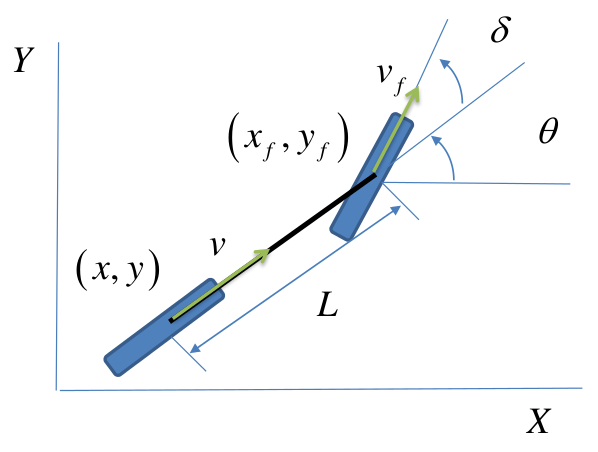
\includegraphics[width=0.6\textwidth]{images/bicycle_model.png}
	\caption{Bicycle in World Frame}
	\label{fig:bicycle}
\end{figure}

Motion of front wheel:

\begin{align}
	x_{f} &= x + L \cos(\theta) \\
	y_{f} &= y + L \sin(\theta) \\
 	\begin{bmatrix}
        x_{f, t} \\
        y_{f, t} \\
    \end{bmatrix}  
    &=
    \begin{bmatrix}
	    x_{f, t - 1} + v_{f, t} \cos(\theta_{f, t - 1} + \delta_{t}) dt \\
		y_{f, t - 1} + v_{f, t} \sin(\theta_{f, t - 1} + \delta_{t}) dt \\
    \end{bmatrix}
\end{align}

Motion of rear wheel:

\begin{align}
 	\begin{bmatrix}
        x_{r, t} \\
        y_{r, t} \\
    \end{bmatrix}  
    &=
    \begin{bmatrix}
	    x_{r, t - 1} + v_{r, t} \cos(\theta_{r, t - 1}) dt \\
		y_{r, t - 1} + v_{r, t} \sin(\theta_{r, t - 1}) dt \\
    \end{bmatrix}
\end{align}

At current we have a motion model for both the front and the rear wheel of the bicycle, however we can simplify it using the Instantaneous Center of Rotation to combine both the front and rear wheel together.

\begin{figure}[H]
	\centering
	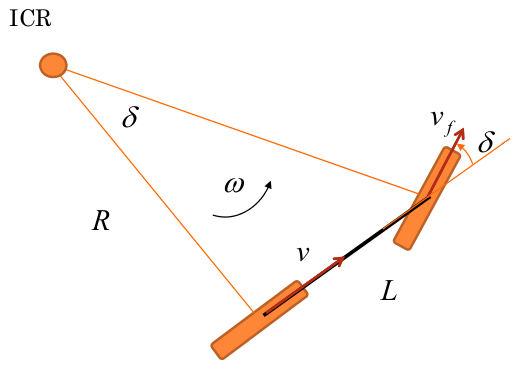
\includegraphics[width=0.6\textwidth]{images/bicycle_icr.png}
	\caption{Simplifying the Bicycle Model with ICR}
	\label{fig:bicycle_icr}
\end{figure}

From Fig~\ref{fig:bicycle_icr} we can derive the relationship between the steering angle $\delta$ relative to the bicycle's heading:

\begin{equation}
	\label{eq:icr_steering_angle}
	\tan(\delta) = \dfrac{L}{R}
\end{equation}

Further, we know that the angular velocity $\omega$ from the point ICR of both the front and rear wheel is:

\begin{equation}
	\label{eq:icr_angluar_velocity}
	\omega = \dfrac{v \tan(\delta)}{L} = \dfrac{v}{R}
\end{equation}

Now that we have the angular velocity of the bicycle over time, the bicycle's change in heading over time is simply:

\begin{equation}
	\theta_{t} = \theta_{t - 1} + \dfrac{v_{t} \tan(\delta_{t})}{L} dt
\end{equation}

For the complete motion model of the bicycle we have:

\begin{align}
 	\begin{bmatrix}
        x_{t} \\
        y_{t} \\
        \theta_{t}
    \end{bmatrix}  
    &=
    \begin{bmatrix}
	    x_{t - 1} + v_{t} \cos(\theta_{t - 1}) dt \\
		y_{t - 1} + v_{t} \sin(\theta_{t - 1}) dt \\
		\theta_{t - 1} + \dfrac{v_{t} \tan(\delta_{t})}{L} dt
    \end{bmatrix}
\end{align}

Implementing the bicycle motion model in Matlab and simulating the motion for 20 seconds with the following parameters, we obtain a motion that resembles Fig~\ref{fig:bicycle_20s}.

\begin{itemize}	
	\vspace{-0.4cm}
	\setlength{\itemsep}{0pt}
	\setlength{\parskip}{0pt}
	\setlength{\parsep}{0pt}
	
	\item{Simulation time step $dt$: 0.1s}
	\item{Velocity $v$: $3 \text{ms}^{-1}$}
	\item{Length of bicycle $L$: 0.3m}
	\item{Steering angle $\delta$: $10 - t$ degrees}
	\item{Steering angle limit: $\pm 30$ degrees}
	\item{Standard deviation on $x$ and $y$: 0.02m}
	\item{Standard deviation on $\theta$: 1 degree}
\end{itemize}

\begin{figure}[H]
	\centering
	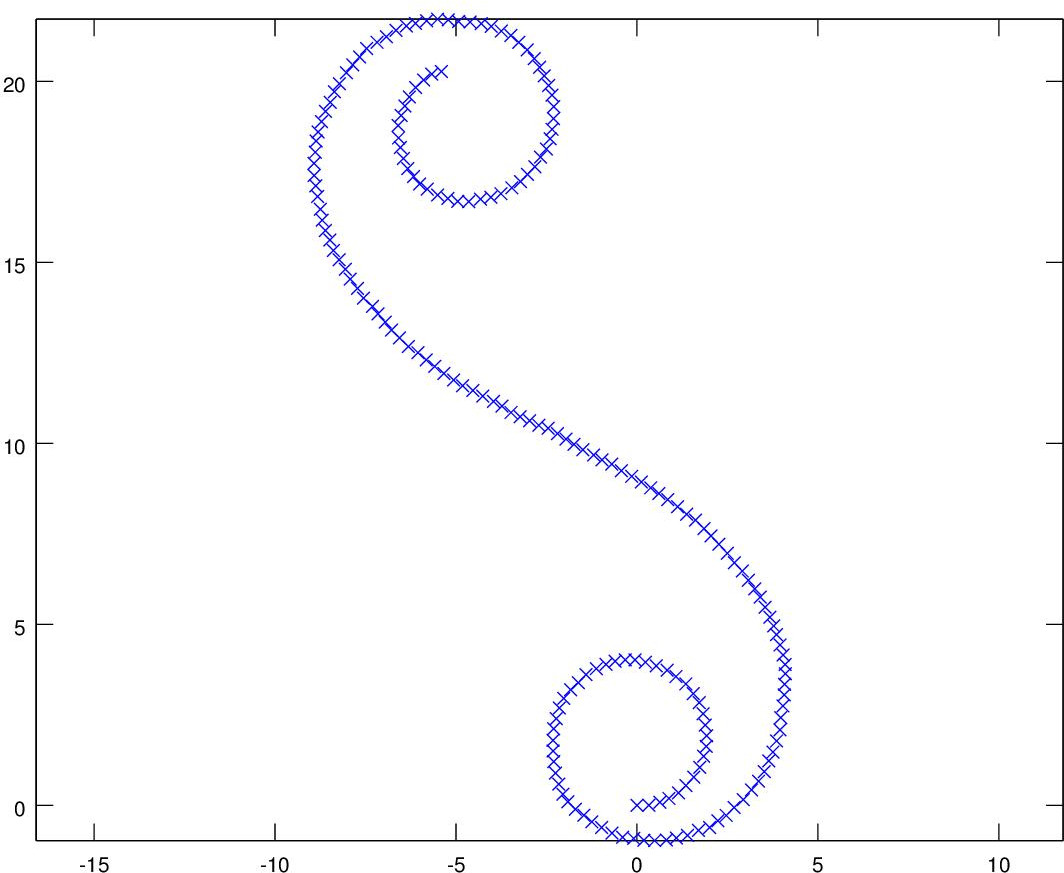
\includegraphics[width=0.7\textwidth]{images/bicycle_motion_20s.jpg}
	\caption{Simulating the Bicycle Model for 20s starting from (0, 0)}
	\label{fig:bicycle_20s}
\end{figure}

Just looking at Fig~\ref{fig:bicycle_20s} we can roughly validate the motion as valid, since the angle starts from +10 and ends at -10 degrees over time (20 seconds).





\newpage
\section{Carrot Controller for Bicycle}

\begin{figure}[H]
	\centering
	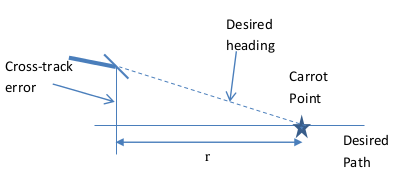
\includegraphics[width=0.6\textwidth]{images/carrot_controller.png}
	\caption{Carrot Controller}
	\label{fig:carrot_controller}
\end{figure}

A carrot controller is a controller that has a carrot point with a fixed distance $r$ on the trajectory line ahead of the closest point on the line to the current robot position.


\newpage
\section{Planner}




\end{document}